% Standalone exporter for presentation PNGs
\documentclass[tikz,border=10pt]{standalone}
\usepackage[T1]{fontenc}
\IfFileExists{newtxtext.sty}{\usepackage{newtxtext}}{}
\usetikzlibrary{positioning,arrows.meta,shapes.geometric,fit,calc,backgrounds}
% Shared TikZ styles for methodology / system diagrams
\definecolor{DiagSlate}{RGB}{32,56,78}
\definecolor{DiagBlue}{RGB}{55,98,140}
\definecolor{DiagTeal}{RGB}{45,125,125}
\definecolor{DiagSoft}{RGB}{232,240,248}
\definecolor{DiagAccent}{RGB}{196,220,236}
\definecolor{DiagWarn}{RGB}{180,110,60}
\definecolor{DiagOk}{RGB}{60,130,90}

\tikzset{
  diag box/.style={
    draw=DiagSlate,
    line width=0.6pt,
    rounded corners=2pt,
    align=center,
    font=\footnotesize\sffamily,
    inner sep=5pt,
    minimum height=0.85cm
  },
  diag start/.style={diag box, fill=DiagSlate, text=white, font=\footnotesize\sffamily\bfseries},
  diag step/.style={diag box, fill=DiagSoft, text=DiagSlate},
  diag model/.style={diag box, fill=DiagAccent, text=DiagSlate, minimum width=2.5cm},
  diag out/.style={diag box, fill=DiagTeal, text=white, font=\footnotesize\sffamily\bfseries},
  diag gate/.style={diag box, fill=DiagWarn!18, text=DiagSlate, draw=DiagWarn},
  diag ok/.style={diag box, fill=DiagOk!18, text=DiagSlate, draw=DiagOk},
  diag arrow/.style={-{Latex[length=2.2mm]}, thick, DiagSlate!80},
  diag label/.style={font=\scriptsize\sffamily, text=DiagSlate!80, align=center}
}


\begin{document}

% 1 methodology pipeline
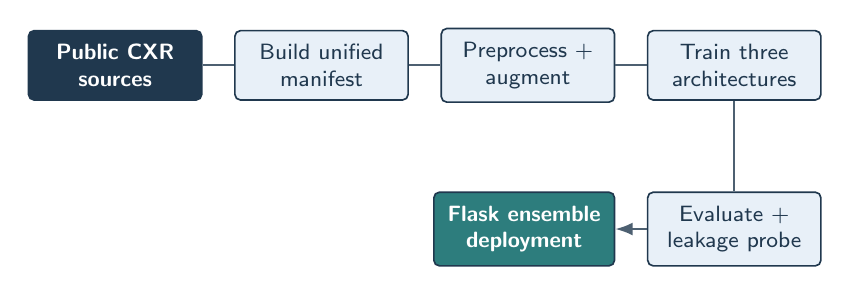
\begin{tikzpicture}[node distance=0.5cm and 0.4cm]
\node[diag start, minimum width=2.2cm] (s1) {Public CXR\\sources};
\node[diag step, right=of s1, minimum width=2.2cm] (s2) {Build unified\\manifest};
\node[diag step, right=of s2, minimum width=2.2cm] (s3) {Preprocess +\\augment};
\node[diag step, right=of s3, minimum width=2.2cm] (s4) {Train three\\architectures};
\node[diag step, below=1.15cm of s4, minimum width=2.2cm] (s5) {Evaluate +\\leakage probe};
\node[diag out, left=of s5, minimum width=2.2cm] (s6) {Flask ensemble\\deployment};
\draw[diag arrow] (s1)--(s2)--(s3)--(s4)--(s5)--(s6);
\end{tikzpicture}

% 2 data unify
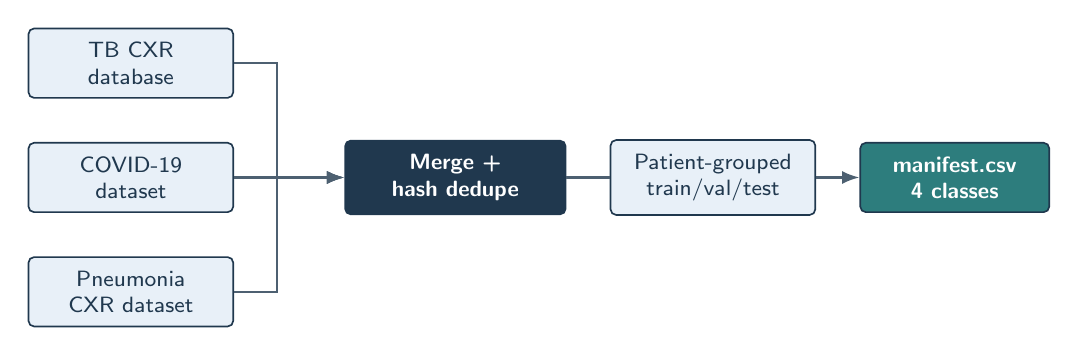
\begin{tikzpicture}[node distance=0.55cm and 0.55cm]
\node[diag step, minimum width=2.6cm] (tb) {TB CXR\\database};
\node[diag step, below=of tb, minimum width=2.6cm] (cov) {COVID-19\\dataset};
\node[diag step, below=of cov, minimum width=2.6cm] (pn) {Pneumonia\\CXR dataset};
\node[diag start, right=1.4cm of cov, minimum width=2.8cm] (merge) {Merge +\\hash dedupe};
\node[diag step, right=of merge, minimum width=2.6cm] (split) {Patient-grouped\\train/val/test};
\node[diag out, right=of split, minimum width=2.4cm] (man) {manifest.csv\\4 classes};
\draw[diag arrow] (tb.east)--++(0.55,0)|-(merge.west);
\draw[diag arrow] (cov)--(merge);
\draw[diag arrow] (pn.east)--++(0.55,0)|-(merge.west);
\draw[diag arrow] (merge)--(split)--(man);
\end{tikzpicture}

% 3 model arch
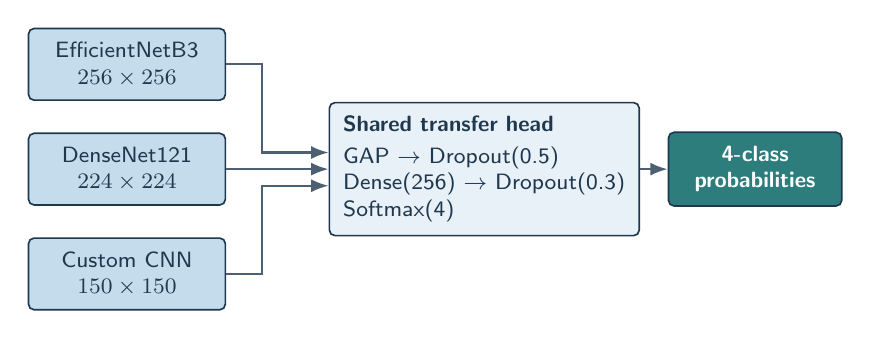
\begin{tikzpicture}[node distance=0.4cm and 0.35cm]
\node[diag model] (eff) {EfficientNetB3\\$256\times256$};
\node[diag model, below=of eff] (den) {DenseNet121\\$224\times224$};
\node[diag model, below=of den] (cnn) {Custom CNN\\$150\times150$};
\node[diag step, right=1.3cm of den, minimum width=3.6cm, align=left] (head) {\textbf{Shared transfer head}\\[2pt]GAP $\rightarrow$ Dropout(0.5)\\Dense(256) $\rightarrow$ Dropout(0.3)\\Softmax(4)};
\node[diag out, right=of head, minimum width=2.2cm] (out) {4-class\\probabilities};
\draw[diag arrow] (eff.east)--++(0.45,0)|-([yshift=6pt]head.west);
\draw[diag arrow] (den)--(head);
\draw[diag arrow] (cnn.east)--++(0.45,0)|-([yshift=-6pt]head.west);
\draw[diag arrow] (head)--(out);
\end{tikzpicture}

% 4 train phases
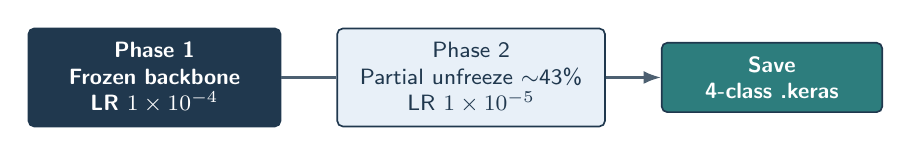
\begin{tikzpicture}[node distance=0.7cm]
\node[diag start, minimum width=3.2cm] (p1) {Phase 1\\Frozen backbone\\LR $1\times10^{-4}$};
\node[diag step, right=of p1, minimum width=3.4cm] (p2) {Phase 2\\Partial unfreeze $\sim$43\%\\LR $1\times10^{-5}$};
\node[diag out, right=of p2, minimum width=2.8cm] (w) {Save\\4-class .keras};
\draw[diag arrow] (p1)--(p2)--(w);
\end{tikzpicture}

% 5 eval flow
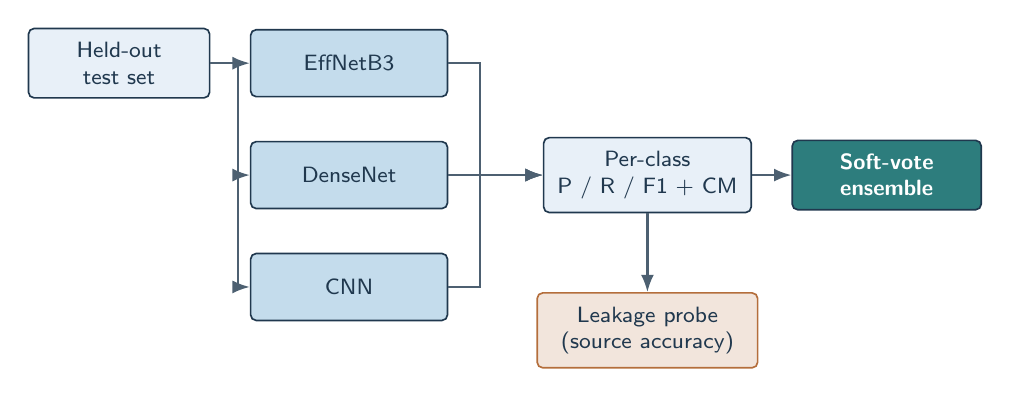
\begin{tikzpicture}[node distance=0.55cm and 0.5cm]
\node[diag step, minimum width=2.3cm] (test) {Held-out\\test set};
\node[diag model, right=of test] (m1) {EffNetB3};
\node[diag model, below=of m1] (m2) {DenseNet};
\node[diag model, below=of m2] (m3) {CNN};
\node[diag step, right=1.2cm of m2, minimum width=2.6cm] (met) {Per-class\\P / R / F1 + CM};
\node[diag out, right=of met, minimum width=2.4cm] (ens) {Soft-vote\\ensemble};
\node[diag gate, below=1.0cm of met, minimum width=2.8cm] (leak) {Leakage probe\\(source accuracy)};
\draw[diag arrow] (test.east)--++(0.35,0)|-(m1.west);
\draw[diag arrow] (test.east)--++(0.35,0)|-(m2.west);
\draw[diag arrow] (test.east)--++(0.35,0)|-(m3.west);
\draw[diag arrow] (m1.east)--++(0.4,0)|-(met.west);
\draw[diag arrow] (m2)--(met);
\draw[diag arrow] (m3.east)--++(0.4,0)|-(met.west);
\draw[diag arrow] (met)--(ens);
\draw[diag arrow] (met)--(leak);
\end{tikzpicture}

% 6 system inference
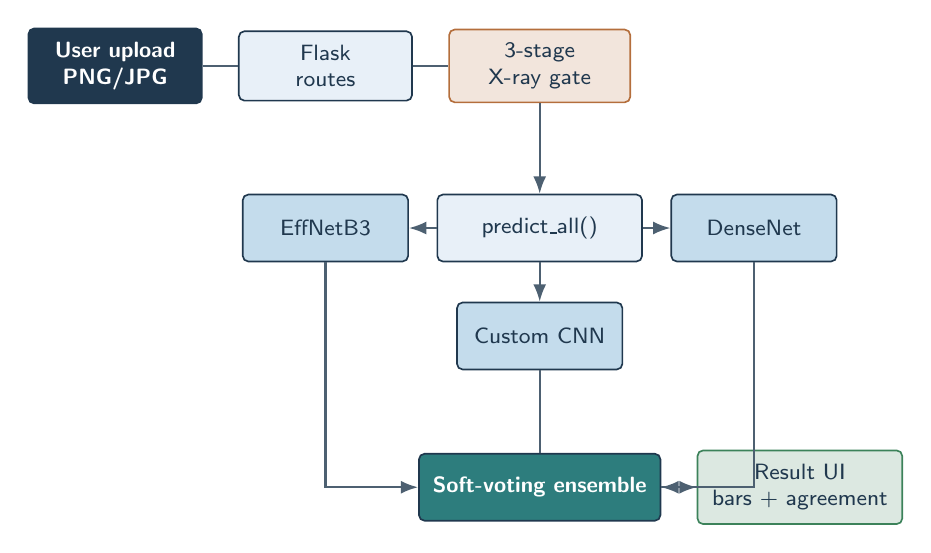
\begin{tikzpicture}[node distance=0.5cm and 0.45cm]
\node[diag start, minimum width=2.2cm] (up) {User upload\\PNG/JPG};
\node[diag step, right=of up, minimum width=2.2cm] (fl) {Flask\\routes};
\node[diag gate, right=of fl, minimum width=2.3cm] (gate) {3-stage\\X-ray gate};
\node[diag step, below=1.15cm of gate, minimum width=2.6cm] (pred) {predict\_all()};
\node[diag model, left=0.35cm of pred, minimum width=2.1cm] (e) {EffNetB3};
\node[diag model, right=0.35cm of pred, minimum width=2.1cm] (d) {DenseNet};
\node[diag model, below=of pred, minimum width=2.1cm] (c) {Custom CNN};
\node[diag out, below=1.05cm of c, minimum width=3.0cm] (ens) {Soft-voting ensemble};
\node[diag ok, right=of ens, minimum width=2.6cm] (ui) {Result UI\\bars + agreement};
\draw[diag arrow] (up)--(fl)--(gate)--(pred);
\draw[diag arrow] (pred)--(e);
\draw[diag arrow] (pred)--(d);
\draw[diag arrow] (pred)--(c);
\draw[diag arrow] (e.south)|-(ens.west);
\draw[diag arrow] (d.south)|-(ens.east);
\draw[diag arrow] (c)--(ens)--(ui);
\end{tikzpicture}

% 7 xray gate
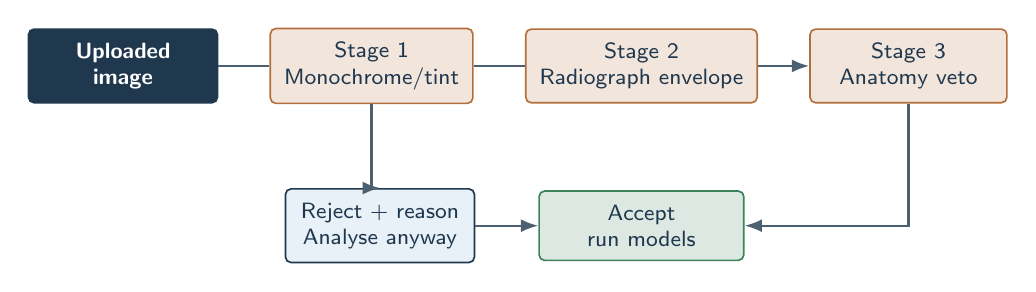
\begin{tikzpicture}[node distance=0.65cm]
\node[diag start, minimum width=2.4cm] (img) {Uploaded\\image};
\node[diag gate, right=of img, minimum width=2.5cm] (g1) {Stage 1\\Monochrome/tint};
\node[diag gate, right=of g1, minimum width=2.5cm] (g2) {Stage 2\\Radiograph envelope};
\node[diag gate, right=of g2, minimum width=2.5cm] (g3) {Stage 3\\Anatomy veto};
\node[diag ok, below=1.1cm of g2, minimum width=2.6cm] (pass) {Accept\\run models};
\node[diag step, left=0.8cm of pass, minimum width=2.4cm] (rej) {Reject + reason\\Analyse anyway};
\draw[diag arrow] (img)--(g1)--(g2)--(g3);
\draw[diag arrow] (g3.south)|-(pass.east);
\draw[diag arrow] (g1.south)|-(rej.north);
\draw[diag arrow] (rej)--(pass);
\end{tikzpicture}

\end{document}
